\setauthor{Isabel Schnalzenberger}

\section{Technologien}

\subsection{Unity}

Unity ist eine leistungsstarke Laufzeit- und Entwicklungsumgebung (IDE) für Spiele, auch als Spiel-Engine (bzw. Gameengine) bekannt, die von Unity Technologies mit Hauptsitz in San Francisco entwickelt wurde. Diese vielseitige Plattform ermöglicht die Erstellung von Spielen und interaktiven 3D-Grafik-Anwendungen für verschiedene Zielplattformen, darunter PCs (Windows und Mac), Spielkonsolen, mobile Geräte und Webbrowser.\footnote{Alle Infos zu Unity stammen von: \cite{UnityDocs}}

\begin{figure} [h t]
    \centering
    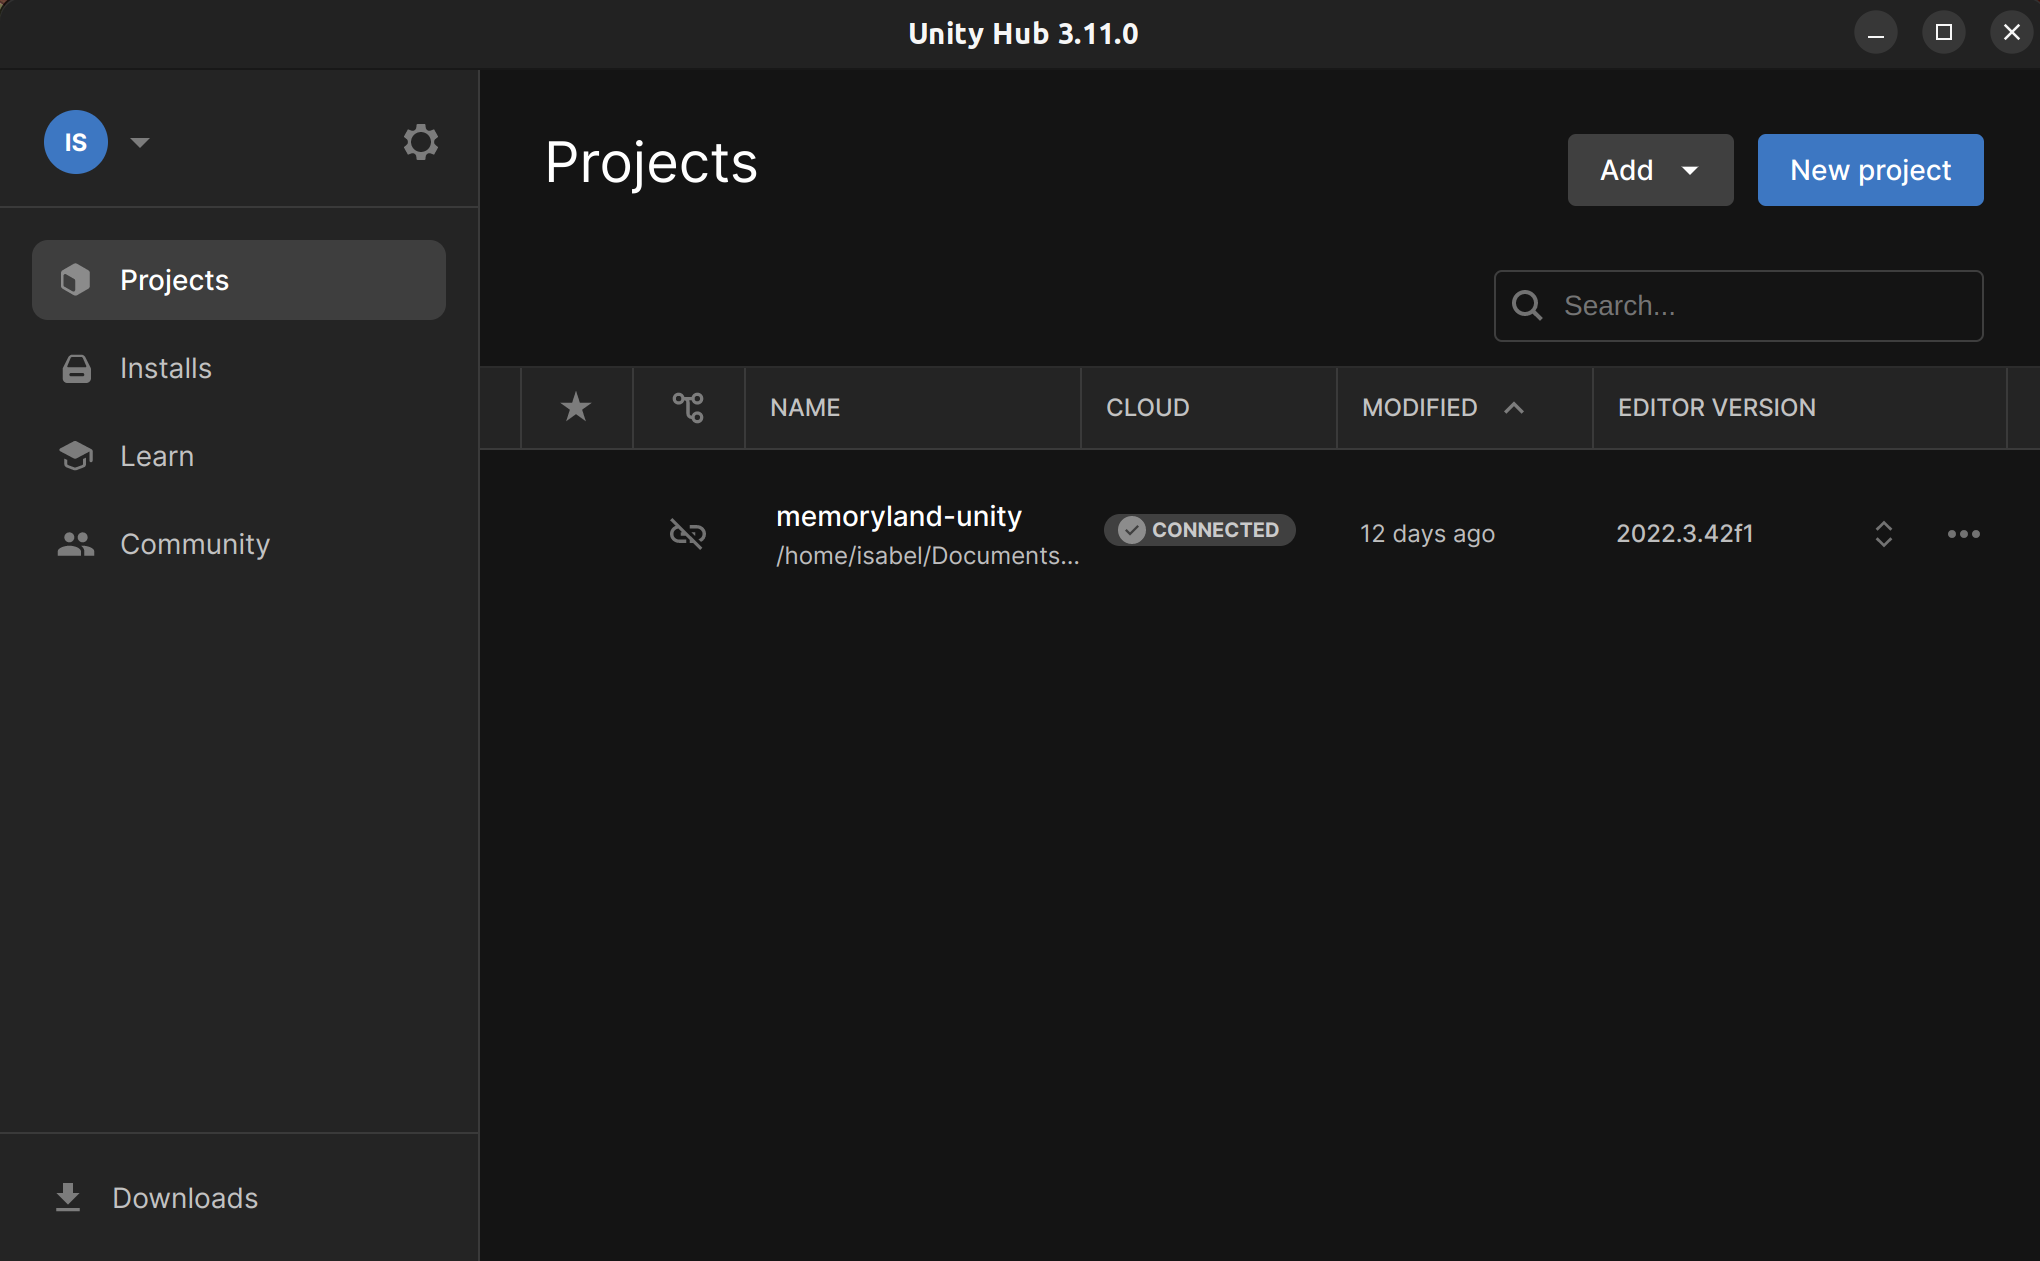
\includegraphics[scale=0.15]{pics/unity-hub.png}
    \caption{Entwicklung in Unity: der Unity-Hub}
    \label{fig:unity-hub}
\end{figure}


\begin{figure} [h t]
    \centering
    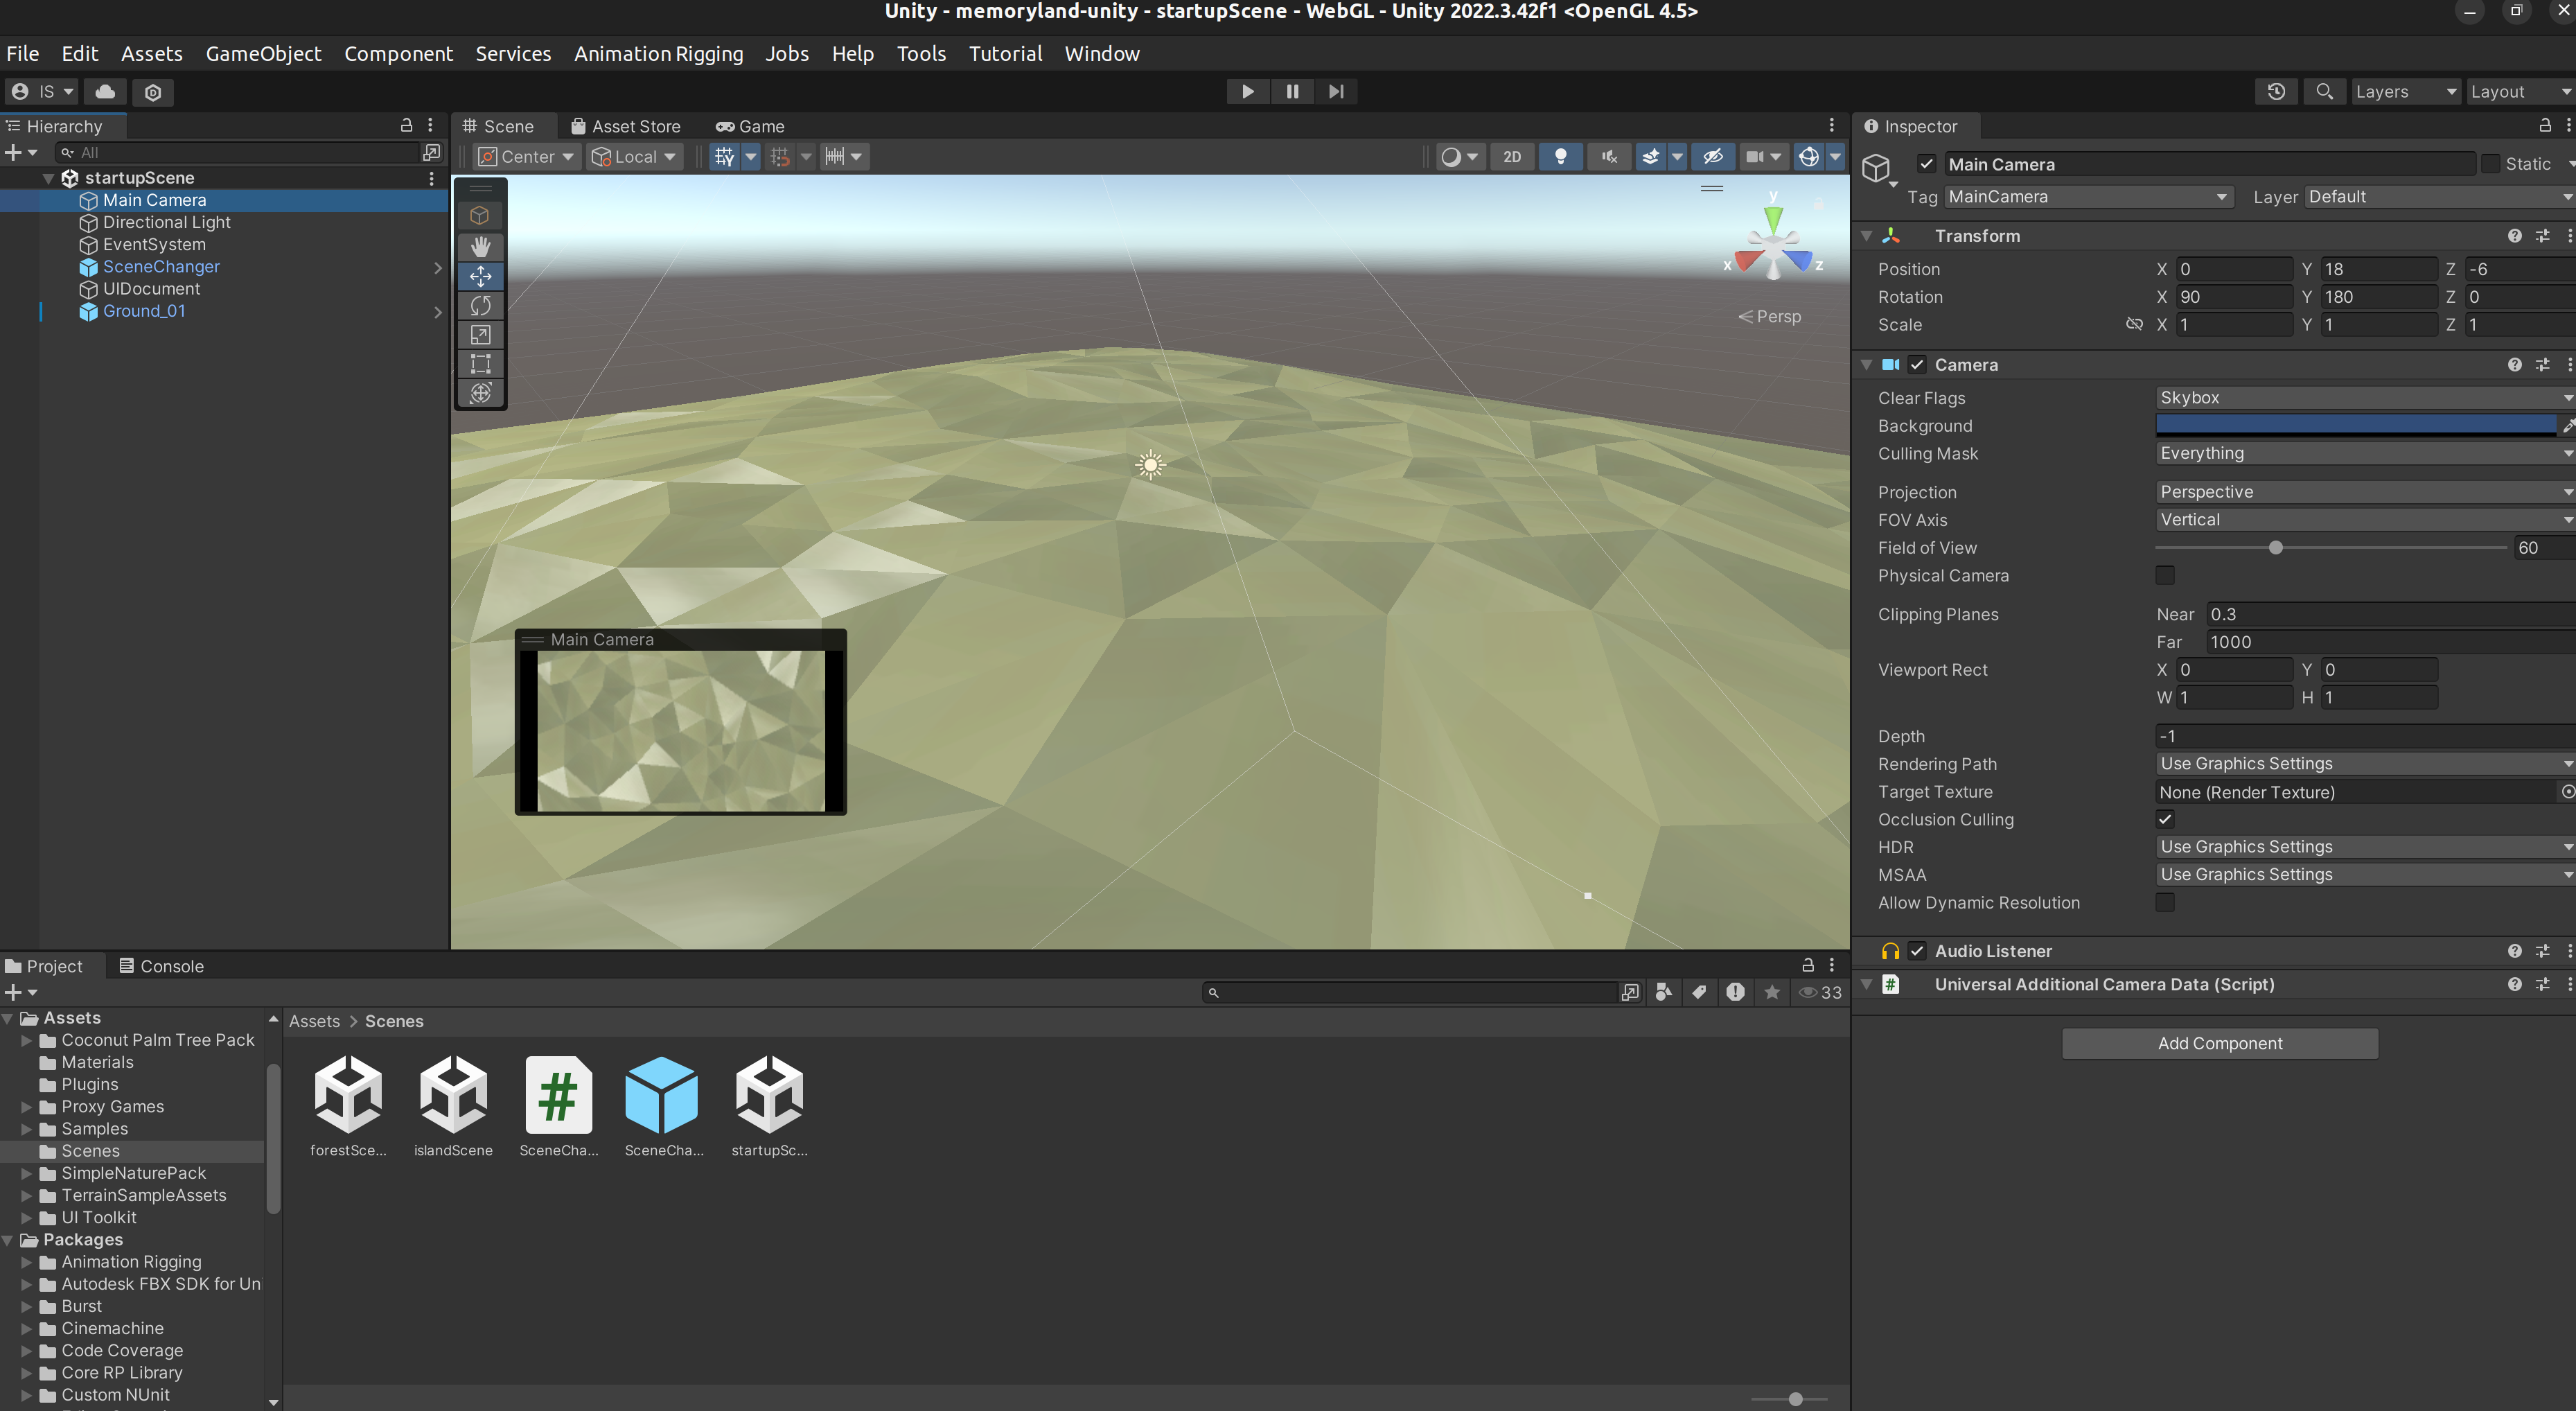
\includegraphics[scale=0.12]{pics/unity-ide.png}
    \caption{Entwicklung in Unity: Die Unity IDE}
    \label{fig:unity-ide}
\end{figure}


Über den Unity-Hub (siehe \ref{fig:unity-hub}) steigt man in den Unity Editor (die IDE, siehe \ref{fig:unity-ide}) ein. Diese Umgebung ist gängigen 3D-Animationsprogrammen und 3D-Entwicklungs-umgebungen nachempfunden. Die Ansicht in der Mitte stellt die aktuelle Sicht auf die Szene dar. Alle gewählten und in der Szene platzierten Objekte befinden sich links in der Hierarchie. Diese wird vor allem für die Auswahl der zu ändernden Objekte verwendet. Auf der rechten Seite befindet sich der Inspektor. Mit seiner Hilfe verändert man einzelne Attribute der sogenannten GameObjects. Es gibt einfach zu ändernde Attribute und veränderliche bzw. durch Programme veränderte Attribute. Die Kombination aus beidem macht Unity so mächtig.\footnote{Alle Infos zum Unity Editor finden sich auch in \cite{UnityDocsEditor}}


Der Entschluss diese Technologie zu verwenden fiel vor allem, weil diese Technologie bereits frühzeitig in unserem Lehrplan enthalten ist und damit umfangreiche Kenntnisse vorhanden waren. Der andere, wesentliche Grund liegt in der Erweiterbarkeit der Umgebung die man in Unity schafft. Die Entwicklungsumgebung ist dergestalt, dass man von Beginn an mit mehreren Scenen im Entwurf gearbeitet hat. Jede Szene (Scene) in Unity spiegelt dabei einen Memorylandtype\footnote{siehe dazu vor allem Abschnitt \ref{sec:memoryland-types}}



\subsection{Visual Studio 2022 und Code}

Der Unity Editor integriert sich mit verschiedenen Source Code Editoren. Die Entwicklung der entsprechenden Klassen weiter unten erfolgte teils in Windows mit Visual Studio 2022 und später auch unter Ubuntu mit Visual Studio Code und anderen Editoren. Die Editoren unterscheiden sich in der Unterstützung der entsprechenden Intellisense und Syntax-Erkennung. Generell ist aber zu sagen, dass die Entwicklung unter Windows angenehmer ist, da hier die volle Bandbreite einer Umgebung zur Verfügung steht, die einerseits die Bibliotheken kennt und die Syntax prüft.



\section{Unity WebGL}

Unity bietet eine besondere Form des Build an: WebGL. Unity WebGL ermöglicht damit die Spiele und interaktiven Anwendungen, die man mit Unity erstellt hat, direkt im Webbrowser aufzurufen, ohne dass zusätzliche Plugins oder Software installiert werden müsste.\footnote{Alle Infos zu Unity WebGL stammen von \cite{UnityDocsWebGL} bzw. \cite{WebGL}}


\begin{wrapfigure}{r}{0.5\textwidth}
    \centering
    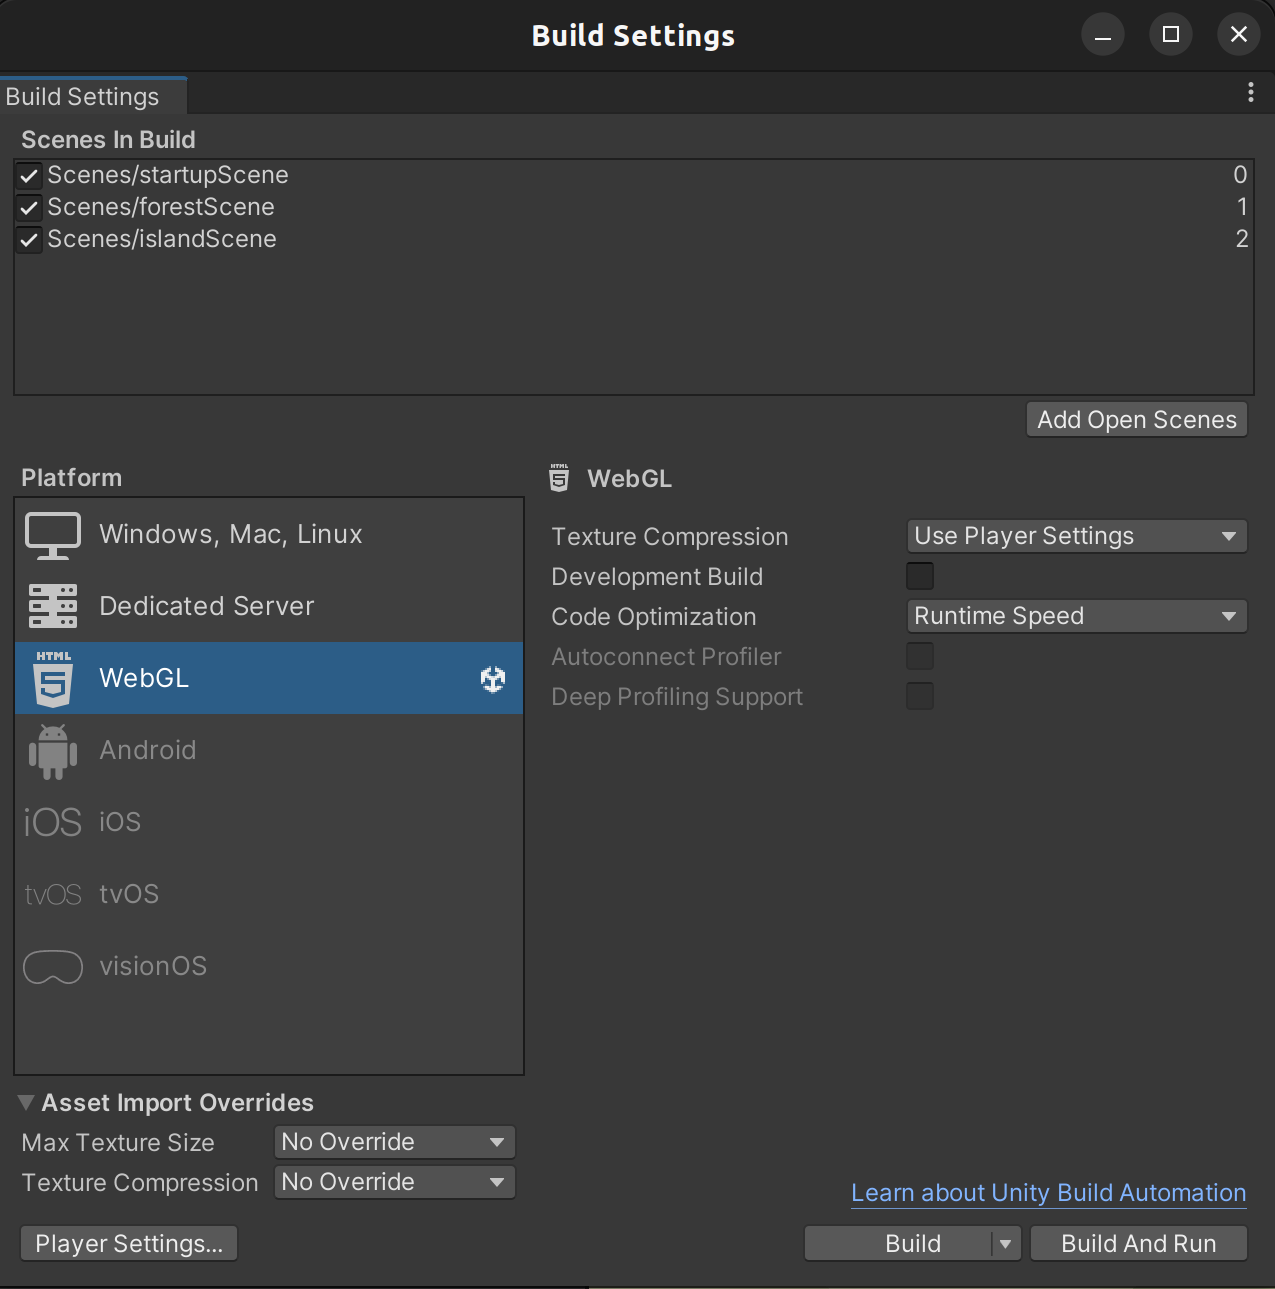
\includegraphics[scale=0.12]{pics/unity-bulid-settings.png}
    \caption{Entwicklung in Unity: Die Unity Build Settings}
    \label{fig:unity-build-settings}



    \centering
    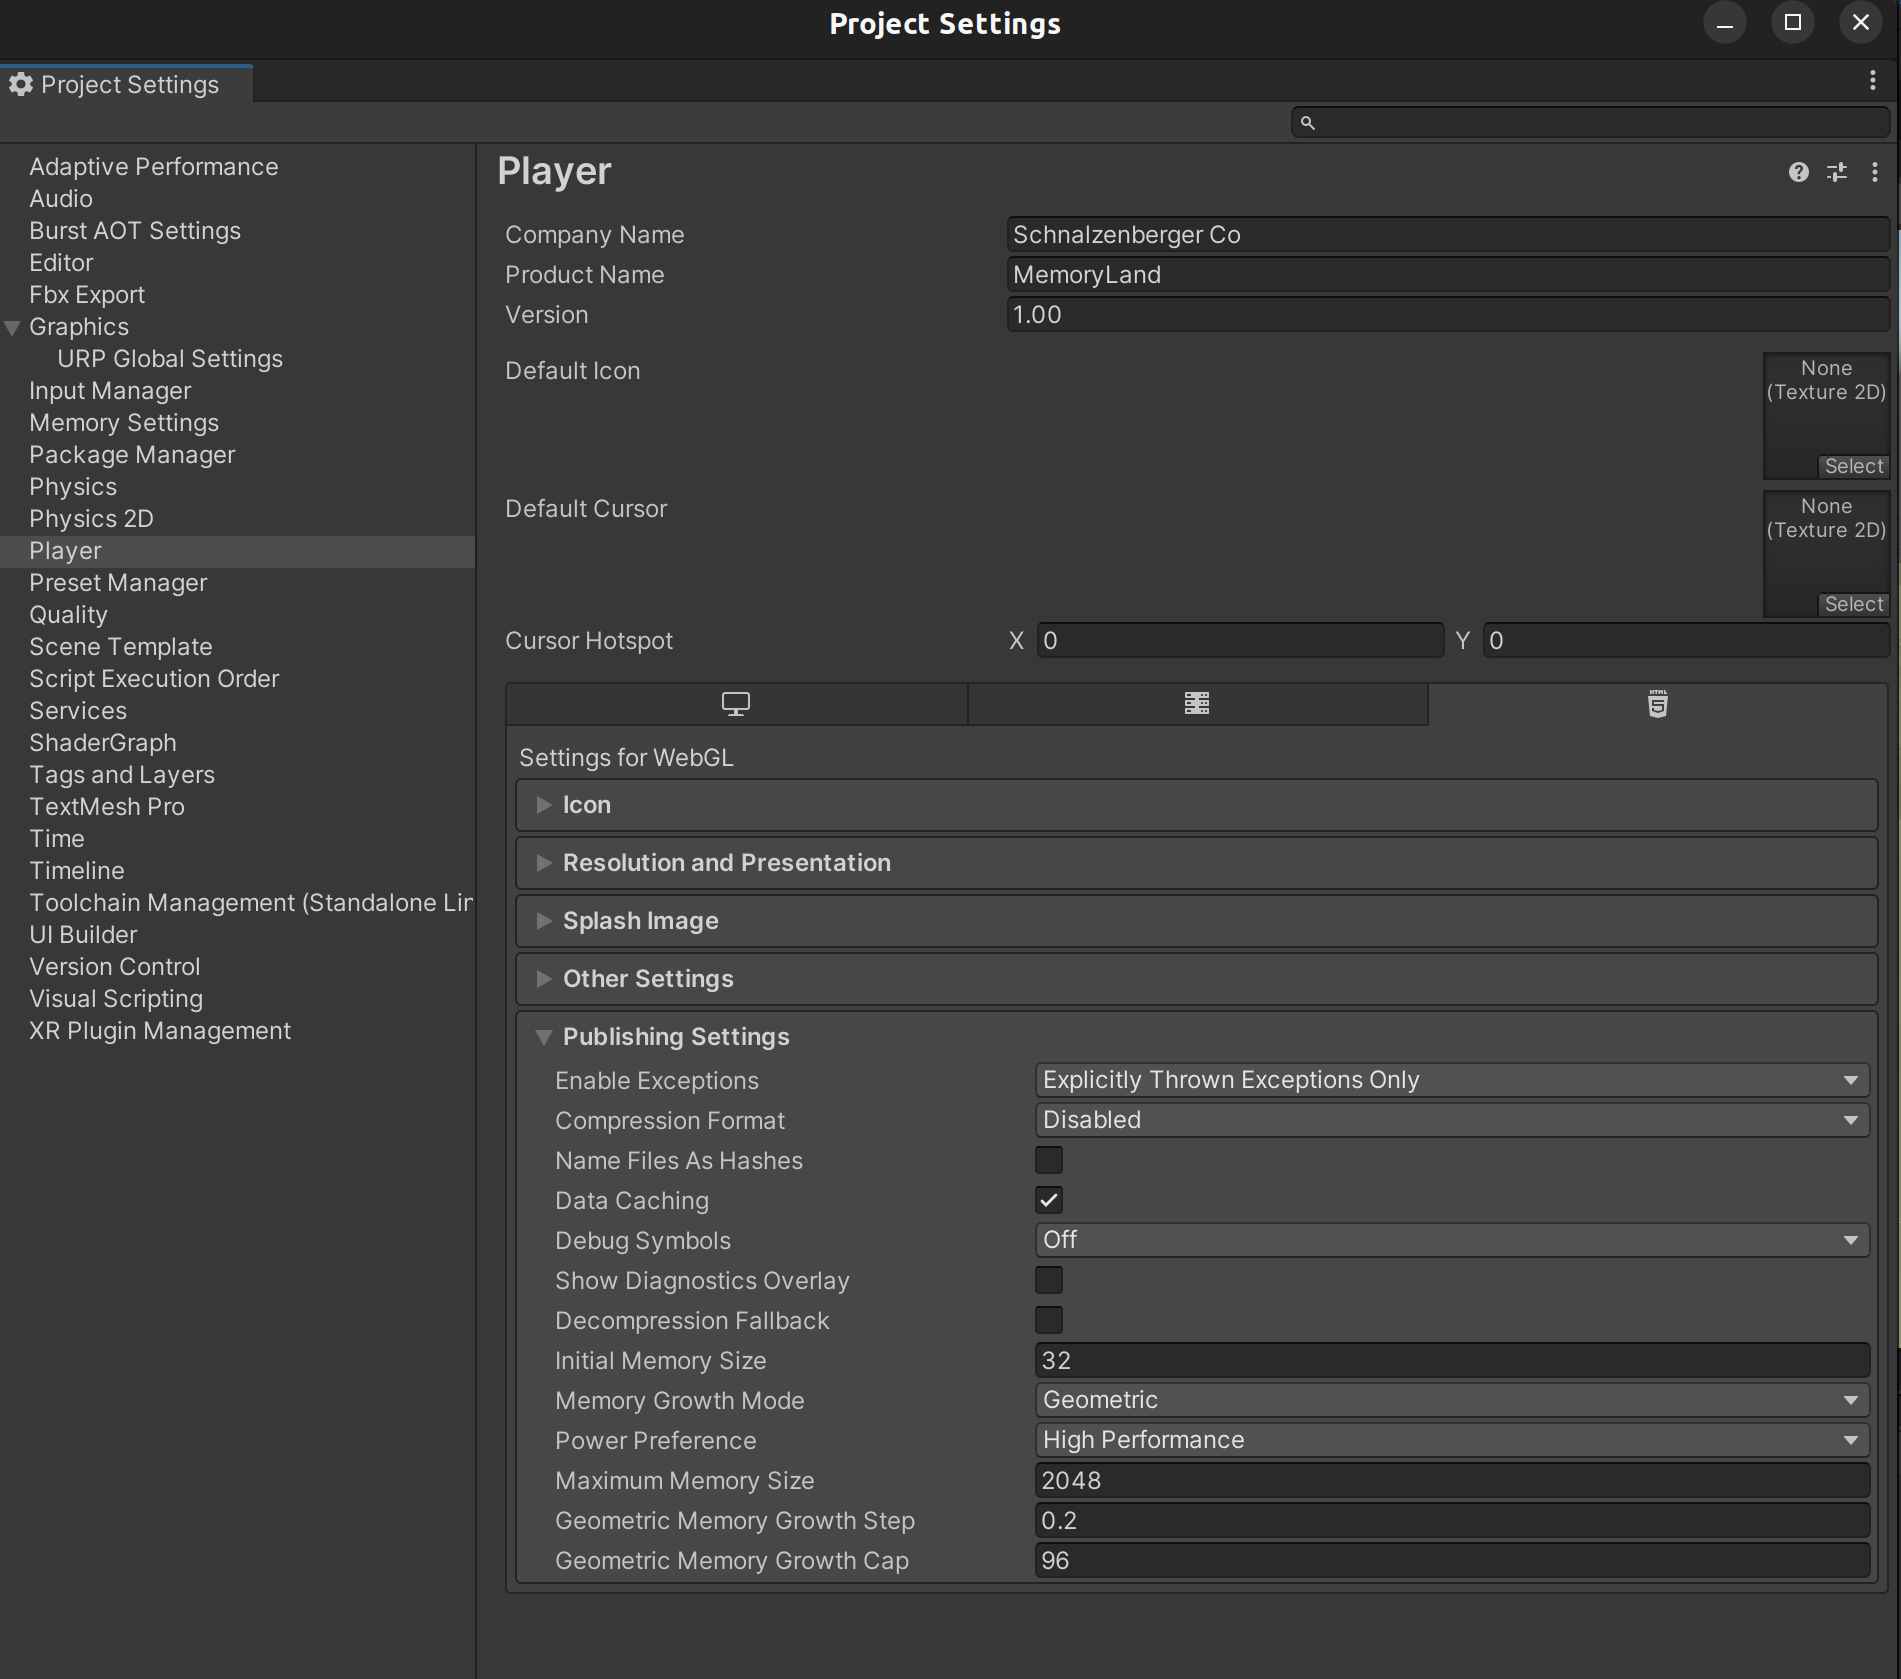
\includegraphics[scale=0.09]{pics/unity-build-webgl-settings.png}
    \caption{Entwicklung in Unity: Die Unity Build Settings für WebGL}
    \label{fig:unity-build-webgl-settings}
\end{wrapfigure}



WebGL (Web Graphics Library) ist eine JavaScript-API, die 3D-Grafiken im Browser rendern kann. Sie basiert dabei auf OpenGL, einer ``shading language'', welche die Beschreibung einer virutellen Umgebung übernimmt. Unity nutzt diese API, um die für Webbrowser optimierte Ausführung von Inhalten zu ermöglichen. WebGL in Unity unterstützt viele gängige Plattformen wie Desktop-Browser (Chrome, Firefox, Safari, etc.) und erlaubt es diesem Projekt die Anwendung Memoryland schnell und einfach online zu verbreiten.

Das Projekt wurde mit den in der Abbildung \ref{fig:unity-build-settings} dargestellten Einstellungen für Unity WebGL entwickelt und der erzeugte JavaScript Code wurde in das Frontend\footnote{siehe Abschnitt \ref{sec:frontend-integration-webgl}}



\section{Implementierung des Unity Projekts}

Im ersten Schritt wurde versucht die .....





\subsection{Url-Parameter}



.....


\subsection{Die Startup Szene}


.....



% startup und load und unity ui toolkit und szenenwechsel


\subsection{Einfügen von Images}

......




\section{Erstellung von neuen Memoryland-Typen}

......

\subsection{Die Wald-Szene}

Die Erstellung der Wald-Szene war am schwierigsten, da die ersten Entwürfe und die Ideenfindung über diese Szene erfolgte. Es wurde versucht einerseits eine ansprechende und umfangreiche Waldumgebung zu erzeugen. Die Idee, die hinter einer Waldumgebung stand, ist die Darstellung von Fotos und Erinnerungen aus einer Wanderung im Grünen.

Diese Wanderungserinnerung ließ sich für die Autoren am klarsten durch einen Wald abrufen. Ein Wald mit vielen verschiedenen Bäumen und Blumen. Die Szene wurde also entsprechend aufgebaut. Dabei wurde zuerst teilweise auf Beispiele aus dem Unterricht zurückgegriffen. Diese waren aber leider zu detailreich, um auch wirklich auf allen Zielplattformen dargestellt werden zu können. Die Anzahl der Details wurde daher reduziert und auf  .....


\subsection{Die Insel-Szene}

Nachdem die umfangreichen Tests der Integration der Unity WebGL in das Frontend und das laufende Backend erfolgreich waren, stand nun der Weg offen für die Entwicklung einer weiteren Ferien-Umgebungs-Szene. Die   

\subsection{Erweiterbarkeit}

Nach dem vorliegenden Konzept kann nun um beliebige Szenen erweitert werden. Die Szenen müssen mehreren Entwicklungsanforderungen und Grundkonzepten folgen. Die größte Freiheit besteht jedoch darin, dass die Szenen zukünftig auch so programmiert werden können, dass man sich beispielsweise selbständig durch die Szene beweigen könnte.

Erste Voraussetzung ist die Darstellung der Bilder mit Hilfe der bereits .......


